\documentclass[10pt,aspectratio=43,mathserif,table]{beamer} 
%  设置为 Beamer 文档类型,设置字体为 10pt,长宽比为16:9,数学字体为 serif 风格
\batchmode

\usepackage{graphicx}
\usepackage{subfig}
\usepackage{animate}
\usepackage{hyperref}
\usepackage{diagbox} % 表头斜线分区
% 导入一些用到的宏包
\usepackage{amsmath,bm,amsfonts,amssymb,enumerate,epsfig,bbm,calc,color,ifthen,capt-of,multimedia,hyperref}
\usefonttheme{serif}
\usepackage{mathptmx}
\usepackage{xeCJK} %导入中文包
%\setCJKmainfont{SimHei} %字体采用黑体  Microsoft YaHei
%\setmonofont{Courier New}
%\setCJKmainfont[AutoFakeBold = {2.15},ItalicFont={KaiTi}]{SimSun}
%\setCJKfamilyfont{xw}{STXinwei}

%\setsansfont{Microsoft YaHei}

%\setsansfont{Arial}


\usetheme{Berlin} %主题
\setbeamertemplate{page number in head/foot}[pagenumber]
%\usecolortheme{sustech} %主题颜色

\usepackage[ruled,linesnumbered]{algorithm2e}

\usepackage{fancybox}
\usepackage{xcolor}
% \usepackage{times}
\usepackage{listings}

\usepackage{booktabs}
\usepackage{colortbl}

\newcommand{\Console}{Console}
\lstset{ %
	backgroundcolor=\color{white},   % choose the background color
	basicstyle=\footnotesize\rmfamily,     % size of fonts used for the code
	columns=fullflexible,
	breaklines=true,                 % automatic line breaking only at whitespace
	captionpos=b,                    % sets the caption-position to bottom
	tabsize=4,
	commentstyle=\color{mygreen},    % comment style
	escapeinside={\%*}{*)},          % if you want to add LaTeX within your code
	keywordstyle=\color{blue},       % keyword style
	stringstyle=\color{mymauve}\ttfamily,     % string literal style
	numbers=left, 
	%	frame=single,
	rulesepcolor=\color{red!20!green!20!blue!20},
	% identifierstyle=\color{red},
	language=c
}


\definecolor{mygreen}{rgb}{0,0.6,0}
\definecolor{mymauve}{rgb}{0.58,0,0.82}
\definecolor{mygray}{gray}{.9}
\definecolor{mypink}{rgb}{.99,.91,.95}
\definecolor{mycyan}{cmyk}{.3,0,0,0}

%题目,作者,学校,日期
\title{Phase Plane}
%\subtitle{\fontsize{9pt}{14pt}\textbf{跨临界分岔}}
\author{Speaker: Yichen Lu\quad \newline  \newline \quad }
\institute{\fontsize{8pt}{14pt}}
\date{\today}
\newcommand{\concept}{Phase Plane}

%学校Logo
%\pgfdeclareimage[height=0.5cm]{sustech-logo}{sustech-logo.pdf}
%\logo{\pgfuseimage{sustech-logo}\hspace*{0.3cm}}

\AtBeginSection[]
{
	\begin{frame}<beamer>
	\frametitle{\textbf{Contents}}
	\tableofcontents[currentsection]
\end{frame}
}
% \beamerdefaultoverlayspecification{<+->}
% -----------------------------------------------------------------------------
\begin{document}
% -----------------------------------------------------------------------------

\frame{\titlepage}

% \section[Contents]{}   %目录
% \begin{frame}{Contents}
% \tableofcontents
% \end{frame}

% -----------------------------------------------------------------------------
\section{Phase Portraits} % 相图

\begin{frame}
    % 到这一章,我们开始研究的是二维的非线性系统,相平面中向量场的一般表达式为
    The general form of a vector field on the phase plane is
    $$
    \begin{array}{c}
        \dot{x}_1=f_1\left( x_1,x_2 \right)\\
        \dot{x}_2=f_2\left( x_1,x_2 \right)\\
    \end{array}
    $$

    This system can be written more compactly in vector notation as
    % 利用向量的定义,这个系统可以被表达为如下简洁的向量形式

    $$\dot{\mathbf{x}}=\mathbf{f}\left( \mathbf{x} \right) $$

    where 
    $\begin{cases}
        \mathbf{x}=\left( x_1,x_2 \right)\\
        \mathbf{f}\left( \mathbf{x} \right) =\left( f_1\left( \mathbf{x} \right) ,f_2\left( \mathbf{x} \right) \right)\\
    \end{cases}$
\end{frame}

\begin{frame}
    % 对于非线性系统,轨迹的解析解通常无法找到。即便能找到解析解,也常因其太复杂而难以洞察其本质。因此,一般的研究目标是直接根据f(x)的性质来描绘系统的相图。下面就是一张相图的例子。
    \begin{figure}
		\centering
		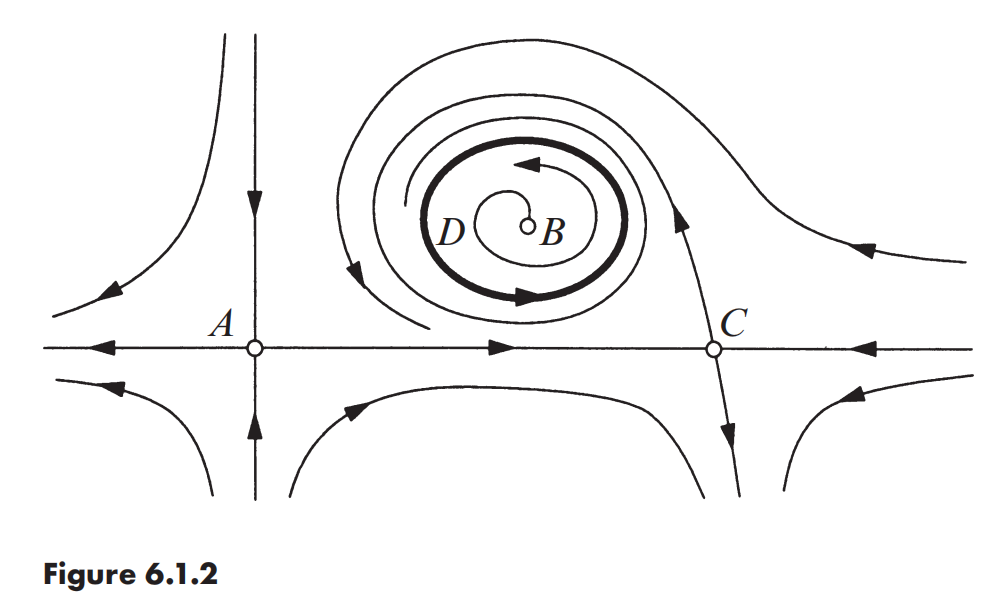
\includegraphics[width=0.7\linewidth]{f612.jpg}
	\end{figure}

    \begin{itemize}
        \item Fixed Points: $\dot{\mathbf{x}}=0$, $A, B$ and $C$
        \item Closed orbits: $\mathbf{x}(t+T)=\mathbf{x}(t)$, $D$
        \item The arrangement of trajectories near the fixed points and closed orbits.
        % 处于不动点及闭轨附近轨迹的排列
        \item The stability or instability of the fixed points and closed orbits.
        % 不动点和闭轨的稳定性或不稳定性
    \end{itemize}
\end{frame}

\begin{frame}
    % 我们考虑这样一个系统
    $$
    \begin{aligned}
        \dot{x}&=x+e^{-y}\\
        \dot{y}&=-y\\
    \end{aligned}
    $$
    \begin{itemize}
        % 首先先来看下不动点,由于y的导数只与y有关,因此y的解析解可以直接求出,y=0,因此不动点只有一个,即x=0,y=0
        \item Fixed Points: $\left( x^*,y^* \right) =\left( -1,0 \right)$ 
        \item Stability: since the solution to $y$ is $y\left( t \right) =y_0e^{-t}$, $y\left( t \right) \rightarrow 0$ when $t\rightarrow \infty$. Hence $e^{-y} \rightarrow 1$, now $\dot{x} \approx x + 1$, this has exponentially growing solutions, unstable.
    \end{itemize}
    
\end{frame}

\begin{frame}
    \textbf{nullclines}: the curves where $\dot{x} = 0$ either or $\dot{y} = 0$. 

    \begin{figure}
		\centering
		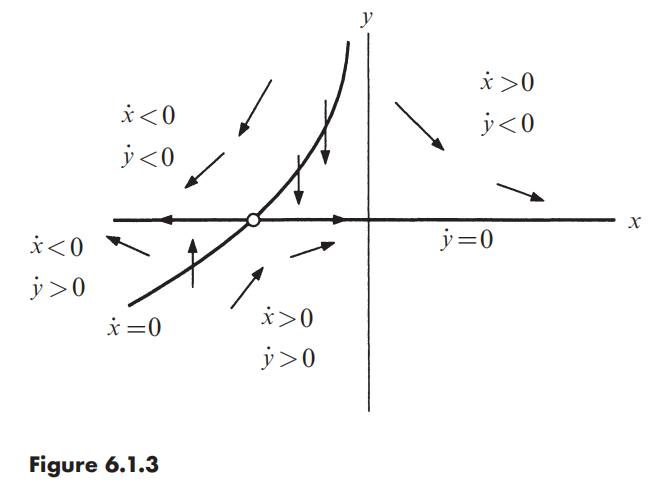
\includegraphics[width=0.7\linewidth]{f613.jpg}
	\end{figure}
\end{frame}

\begin{frame}
    \begin{figure}
		\centering
		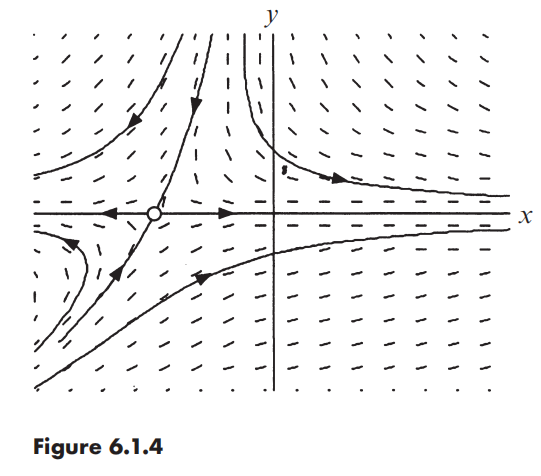
\includegraphics[width=0.7\linewidth]{f614.jpg}
	\end{figure}
\end{frame}

\section{Existence, Uniqueness, and Topological Consequences}

\begin{frame}
    \begin{figure}
        \centering
        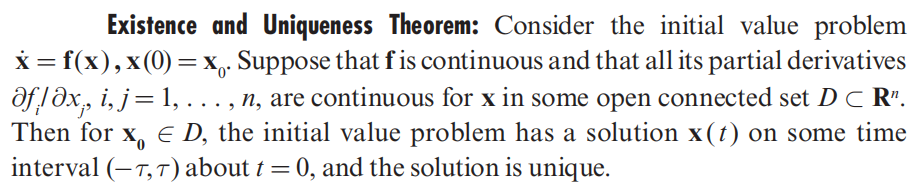
\includegraphics[width=\linewidth]{Existence and Uniqueness Theorem.jpg}
    \end{figure}
    % 也就是说,如果f是连续可微的,那么就能够证明解是存在且唯一的.

    \begin{figure}
        \centering
        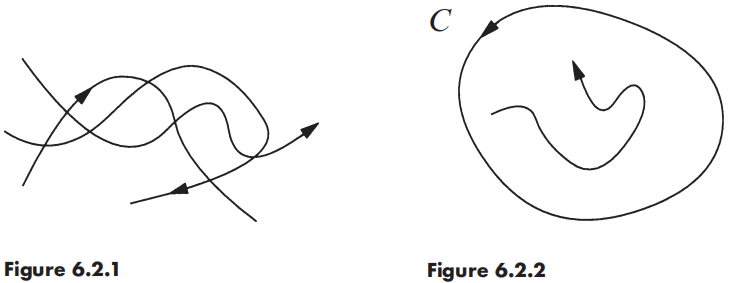
\includegraphics[width=0.8\linewidth]{f621_622.jpg}
    \end{figure}
\end{frame}

\section{Fixed Points and Linearization} % 不动点与线性化



\begin{frame}
    % 前面我们在研究一维非线性系统的时候,就用过线性化的方法来分析不动点的稳定性。这里我们也可以用类似的方法来分析二维系统中的不动点的稳定性。上一节中我们学习了二维的线性系统,我们的目标是将非线性系统转化为线性系统的形式
    $$
    \begin{array}{c}
        \dot{x}=f\left( x,y \right)\\
        \dot{y}=g\left( x,y \right)\\
    \end{array}
    $$

    Suppose that $(x^*,y^*)$ is a fixed point, i.e.,
    $$
    f\left( x^*,y^* \right) =0, g\left( x^*,y^* \right) =0
    $$
    Small disturbance:
    $$
    u=x-x^*,v=y-y^*
    $$


    \begin{figure}
        \centering
        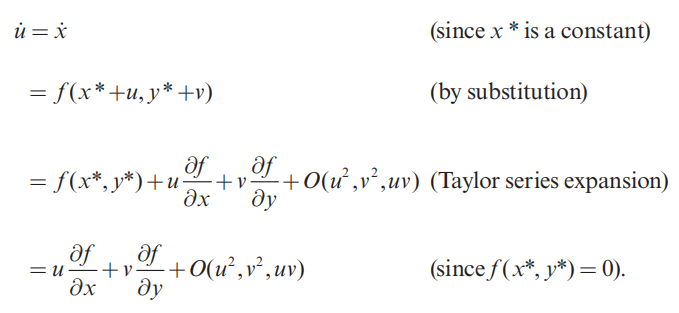
\includegraphics[width=0.8\linewidth]{Linearization.png}
    \end{figure}
\end{frame}

\begin{frame}
    $$
    \left( \begin{array}{c}
        \dot{u}\\
        \dot{v}\\
    \end{array} \right) =\left( \begin{matrix}
        \frac{\partial f}{\partial x}&		\frac{\partial f}{\partial y}\\
        \frac{\partial g}{\partial x}&		\frac{\partial g}{\partial y}\\
    \end{matrix} \right) \left( \begin{array}{c}
        u\\
        v\\
    \end{array} \right) +O\left( u^2,v^2,uv \right) 
    $$
    \textbf{Jacobian matrix} at the fixed point $(x^*,y^*)$:
    $$
    A=\left( \begin{matrix}
        \frac{\partial f}{\partial x}&		\frac{\partial f}{\partial y}\\
        \frac{\partial g}{\partial x}&		\frac{\partial g}{\partial y}\\
    \end{matrix} \right) _{\left( x^*,y^* \right)}
    $$
    \textbf{linearized system}:
    $$
    \left( \begin{array}{c}
        \dot{u}\\
        \dot{v}\\
    \end{array} \right) =\left( \begin{matrix}
        \frac{\partial f}{\partial x}&		\frac{\partial f}{\partial y}\\
        \frac{\partial g}{\partial x}&		\frac{\partial g}{\partial y}\\
    \end{matrix} \right) \left( \begin{array}{c}
        u\\
        v\\
    \end{array} \right) 
    $$

\end{frame}

\begin{frame}{The Effect of Small Nonlinear Terms}
    Is it really safe to neglect the quadratic terms?
    \newline 
    \newline 
    Andronov et al.(1973) showed that the answer is yes: 
    
    \textbf{~~~~~ as long as the fixed point for the linearized system is not one of the borderline cases (centers, degenerate nodes, stars, or non-isolated fixed points)}
    % 只要线性表达式的不动点不是5.2节中讨论的边界情形(中心、退化结点、星形结点或非孤立不动点)中的一类,那么答案就是肯定的

    \begin{figure}
        \centering
        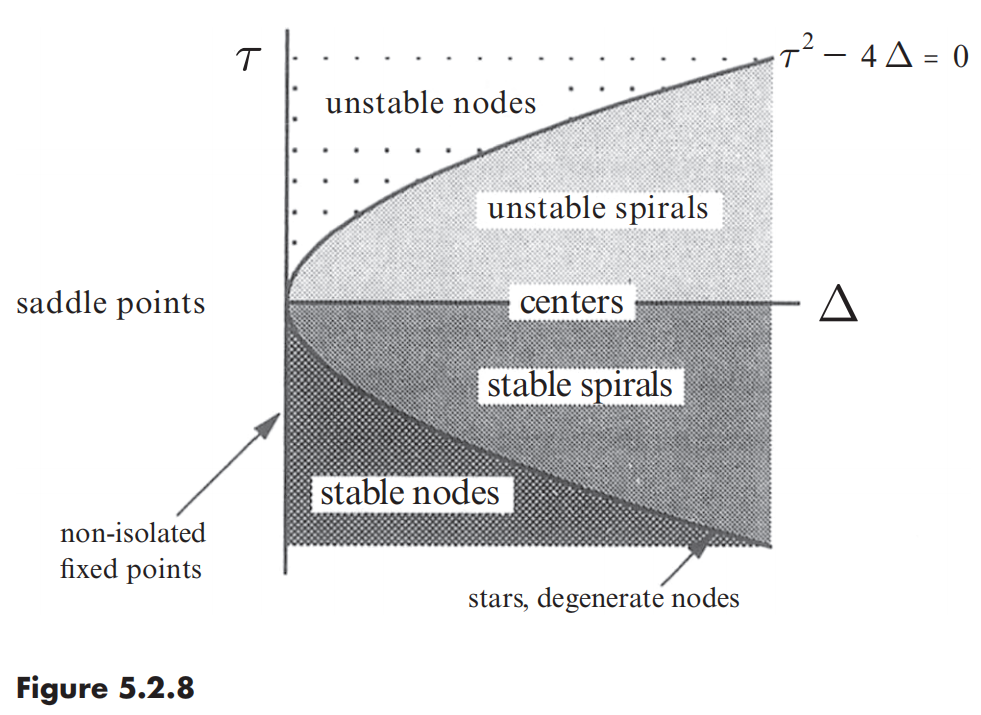
\includegraphics[width=0.6\linewidth]{f528.jpg}
    \end{figure}
    
\end{frame}

\begin{frame}
    $$
    \begin{aligned}
        \dot{x}&=-x+x^3\\
        \dot{y}&=-2y\\
    \end{aligned}
    $$

    $$
    A=\left( \begin{matrix}
        -1+3x^2&		0\\
        0&		-2\\
    \end{matrix} \right) 
    $$

    At $(0, 0)$, 
    $A=\left( \begin{matrix}
        -1&		0\\
        0&		-2\\
    \end{matrix} \right) $, stable node

    At $(\pm 1, 0)$,
    $A=\left( \begin{matrix}
        2&		0\\
        0&		-2\\
    \end{matrix} \right) $, both saddle points

    \begin{figure}
        \centering
        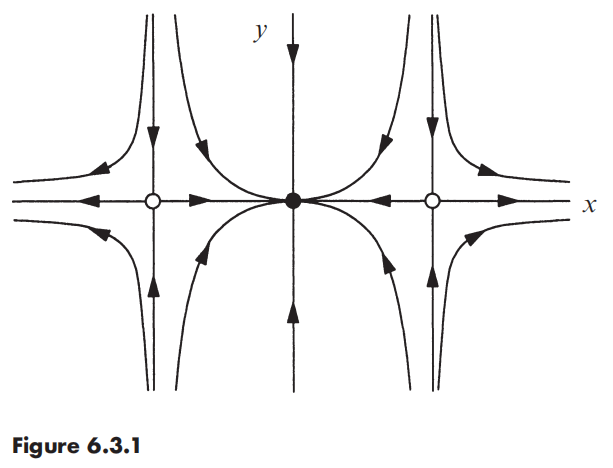
\includegraphics[width=0.5\linewidth]{f631.jpg}
    \end{figure}
\end{frame}

\begin{frame}
    $$
    \begin{aligned}
        \dot{x}&=-y+ax\left( x^2+y^2 \right)\\
        \dot{y}&=x+ay\left( x^2+y^2 \right)\\
    \end{aligned}
    $$

    \textbf{According to Linearization}: $
    A=\left( \begin{matrix}
        0&		-1\\
        1&		0\\
    \end{matrix} \right) 
    $, the origin is a center
    
    \textbf{Polar coordinates} :$
    \begin{cases}
        x=r\cos \theta\\
        y=r\sin \theta\\
    \end{cases}
    $

    $$
    \begin{aligned}
        r^2&=x^2+y^2\\
        r\dot{r}&=x\dot{x}+y\dot{y}\\
        &=x\left( -y+ax\left( x^2+y^2 \right) \right) +y\left( x+ay\left( x^2+y^2 \right) \right)\\
        &=a\left( x^2+y^2 \right) ^2\\
        &=ar^4\\
    \end{aligned}
    $$

    $$
    \begin{cases}
        \dot{r}=ar^3\\
        \dot{\theta}=1\\
    \end{cases}
    $$

\end{frame}

\begin{frame}
    \begin{figure}
        \centering
        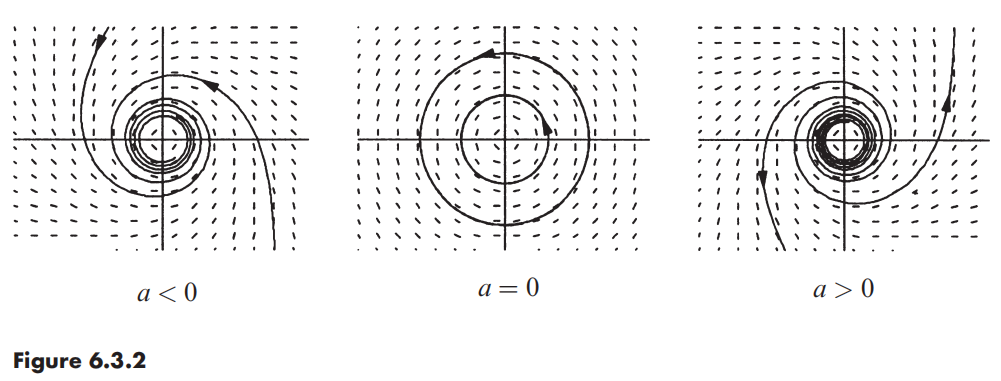
\includegraphics[width=\linewidth]{f632.jpg}
    \end{figure}

    A phase portrait is \textbf{structurally stable} if its topology cannot be changed by an arbitrarily small perturbation to the vector field.
    % 如果相图的拓扑结构不能被向量场一个任意小的扰动所改变,那么这个相图是结构稳定的
\end{frame}

\begin{frame}
    \begin{figure}
        \centering
        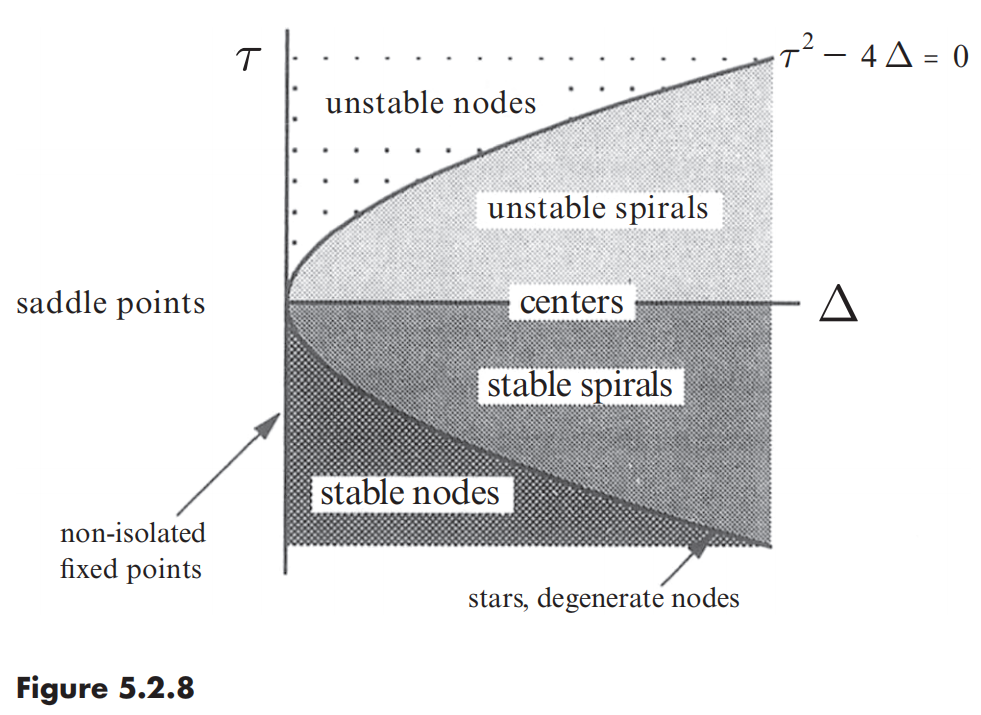
\includegraphics[width=0.55\linewidth]{f528.jpg}
    \end{figure}
    \begin{figure}
        \centering
        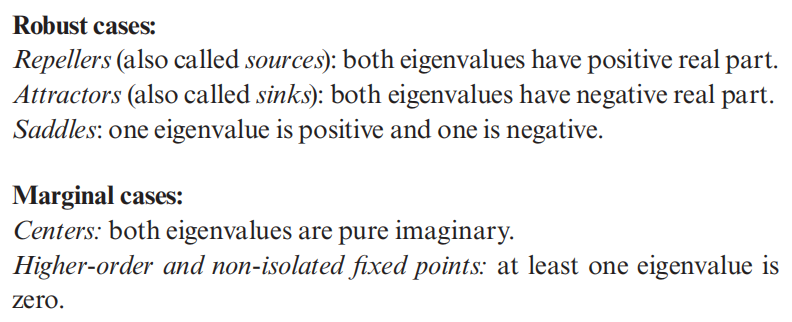
\includegraphics[width=0.7\linewidth]{classify.jpg}
    \end{figure}
\end{frame}

% -----------------------------------------------------------------------------
\end{document}

